%%%%%%%%%%%%%%%%%%%%%%%%%%%%%%%%%%%%%%%%%%%%%%%%%%%%%%%%%%%%%%%%%%%%%%%%%%%%%%%%%%
\begin{frame}[fragile]\frametitle{}
\begin{center}
{\Large Scipy}

(Reference: 
SciPy - Library of scientific algorithms for Python - Johansson )
\end{center}
\end{frame}


%%%%%%%%%%%%%%%%%%%%%%%%%%%%%%%%%%%%%%%%%%%%%%%%%%%%%%%%%%%%%%%%%%%%%%%%%%%%%%%%%%
\begin{frame}[fragile]\frametitle{Introduction}
 \begin{itemize}
  \item The SciPy framework builds on top of the low-level NumPy framework 
  \item Provides a large number of higher-level scientific algorithms. 
  \item Algos:
   \begin{itemize}
  \item The SciPy framework builds on top of the low-level NumPy framework 
  \item Provides a large number of higher-level scientific algorithms. 
  \item Special functions (scipy.special)
  \item Integration (scipy.integrate)
  \item Optimization (scipy.optimize)
  \item Interpolation (scipy.interpolate)
  \item Fourier Transforms (scipy.fftpack)
  \item Signal Processing (scipy.signal)
  \item Linear Algebra (scipy.linalg)
  \item Sparse Eigenvalue Problems (scipy.sparse)
  \item Statistics (scipy.stats)
  \item Multi-dimensional image processing (scipy.ndimage)
  \item File IO (scipy.io)
 \end{itemize}
 \end{itemize}
\end{frame}


%%%%%%%%%%%%%%%%%%%%%%%%%%%%%%%%%%%%%%%%%%%%%%%%%%%%%%%%%%%%%%%%%%%%%%%%%%%%%%%%%%
\begin{frame}[fragile]\frametitle{Special functions}
 \begin{itemize}
  \item A large number of mathematical special functions. 
  \item Eg Bessel functions: jn, yn, jn\_zeros, yn\_zeros
 \end{itemize}
\begin{lstlisting}

n = 0    # order
x = 0.0

# Bessel function of first kind
print "J_%d(%f) = %f" % (n, x, jn(n, x))

x = 1.0
# Bessel function of second kind
print "Y_%d(%f) = %f" % (n, x, yn(n, x))

J_0(0.000000) = 1.000000
Y_0(1.000000) = 0.088257
\end{lstlisting}
\end{frame}



%%%%%%%%%%%%%%%%%%%%%%%%%%%%%%%%%%%%%%%%%%%%%%%%%%%%%%%%%%%%%%%%%%%%%%%%%%%%%%%%%%
\begin{frame}[fragile]\frametitle{Bessel functions}
 \begin{itemize}
  \item A large number of mathematical special functions. 
  \item Eg Bessel functions: jn, yn, jn\_zeros, yn\_zeros
 \end{itemize}
\begin{lstlisting}
x = linspace(0, 10, 100)

fig, ax = plt.subplots()
for n in range(4):
    ax.plot(x, jn(n, x), label=r"$J_%d(x)$" % n)
ax.legend();
\end{lstlisting}
\begin{center}
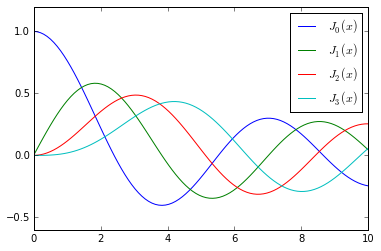
\includegraphics[width=0.5\linewidth,keepaspectratio]{jn}
\end{center}
\end{frame}

%%%%%%%%%%%%%%%%%%%%%%%%%%%%%%%%%%%%%%%%%%%%%%%%%%%%%%%%%%%%%%%%%%%%%%%%%%%%%%%%%%
\begin{frame}[fragile]\frametitle{Numerical Integration}
 \begin{itemize}
  \item  Called numerical quadrature, or simply quadature
  \item quad, dblquad and tplquad for single, double and triple integrals, respectively.
 \end{itemize}
\begin{lstlisting}
from scipy.integrate import quad, dblquad, tplquad
# define a simple function for the integrand
def f(x):
    return x
    
x_lower = 0 # the lower limit of x
x_upper = 1 # the upper limit of x

val, abserr = quad(f, x_lower, x_upper)

print "integral value =", val, ", absolute error =", abserr    
\end{lstlisting}

\end{frame}

%%%%%%%%%%%%%%%%%%%%%%%%%%%%%%%%%%%%%%%%%%%%%%%%%%%%%%%%%%%%%%%%%%%%%%%%%%%%%%%%%%
\begin{frame}[fragile]\frametitle{Numerical Integration}
For simple functions we can use a lambda function (name-less function) instead of explicitly defining a function for the integrand:
\begin{lstlisting}
val, abserr = quad(lambda x: exp(-x ** 2), -Inf, Inf)

print "numerical  =", val, abserr

analytical = sqrt(pi)
print "analytical =", analytical

numerical  = 1.77245385091 1.42026367809e-08
analytical = 1.77245385091
\end{lstlisting}

\end{frame}


%%%%%%%%%%%%%%%%%%%%%%%%%%%%%%%%%%%%%%%%%%%%%%%%%%%%%%%%%%%%%%%%%%%%%%%%%%%%%%%%%%
\begin{frame}[fragile]\frametitle{Ordinary differential equations (ODEs)}
 \begin{itemize}
  \item  An API based on the function odeint, and 
  \item object-oriented API based on the class ode.
  \item Once we have defined the Python function f and array $y_0$ (that is $f$ and $y(0)$ in the mathematical formulation), we can use the odeint function as:
$y_t = odeint(f, y_0, t)$
 \end{itemize}  
\end{frame}

%%%%%%%%%%%%%%%%%%%%%%%%%%%%%%%%%%%%%%%%%%%%%%%%%%%%%%%%%%%%%%%%%%%%%%%%%%%%%%%%%%
\begin{frame}[fragile]\frametitle{Example: double pendulum}
\begin{center}
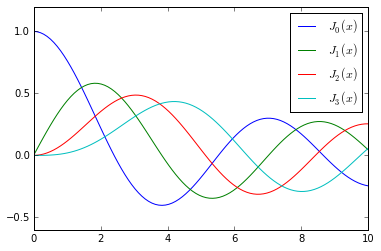
\includegraphics[width=0.8\linewidth,keepaspectratio]{jn}
\end{center}
\end{frame}

%%%%%%%%%%%%%%%%%%%%%%%%%%%%%%%%%%%%%%%%%%%%%%%%%%%%%%%%%%%%%%%%%%%%%%%%%%%%%%%%%%
\begin{frame}[fragile]\frametitle{Example: double pendulum}
\begin{lstlisting}
g = 9.82
L = 0.5
m = 0.1

def dx(x, t):
    """
    The right-hand side of the pendulum ODE
    """
    x1, x2, x3, x4 = x[0], x[1], x[2], x[3]
    
    dx1 = 6.0/(m*L**2) * (2 * x3 - 3 * cos(x1-x2) * x4)/(16 - 9 * cos(x1-x2)**2)
    dx2 = 6.0/(m*L**2) * (8 * x4 - 3 * cos(x1-x2) * x3)/(16 - 9 * cos(x1-x2)**2)
    dx3 = -0.5 * m * L**2 * ( dx1 * dx2 * sin(x1-x2) + 3 * (g/L) * sin(x1))
    dx4 = -0.5 * m * L**2 * (-dx1 * dx2 * sin(x1-x2) + (g/L) * sin(x2))
    
    return [dx1, dx2, dx3, dx4]
\end{lstlisting}
\end{frame}

%%%%%%%%%%%%%%%%%%%%%%%%%%%%%%%%%%%%%%%%%%%%%%%%%%%%%%%%%%%%%%%%%%%%%%%%%%%%%%%%%%
\begin{frame}[fragile]\frametitle{Example: double pendulum}
\begin{lstlisting}
# choose an initial state
x0 = [pi/4, pi/2, 0, 0]

# time coodinate to solve the ODE for: from 0 to 10 seconds
t = linspace(0, 10, 250)

# solve the ODE problem
x = odeint(dx, x0, t)
\end{lstlisting}
\end{frame}

%%%%%%%%%%%%%%%%%%%%%%%%%%%%%%%%%%%%%%%%%%%%%%%%%%%%%%%%%%%%%%%%%%%%%%%%%%%%%%%%%%
\begin{frame}[fragile]\frametitle{Example: double pendulum}
\begin{lstlisting}
# plot the angles as a function of time

fig, axes = plt.subplots(1,2, figsize=(12,4))
axes[0].plot(t, x[:, 0], 'r', label="theta1")
axes[0].plot(t, x[:, 1], 'b', label="theta2")


x1 = + L * sin(x[:, 0])
y1 = - L * cos(x[:, 0])

x2 = x1 + L * sin(x[:, 1])
y2 = y1 - L * cos(x[:, 1])
    
axes[1].plot(x1, y1, 'r', label="pendulum1")
axes[1].plot(x2, y2, 'b', label="pendulum2")
axes[1].set_ylim([-1, 0])
axes[1].set_xlim([1, -1]);
\end{lstlisting}
\end{frame}

%%%%%%%%%%%%%%%%%%%%%%%%%%%%%%%%%%%%%%%%%%%%%%%%%%%%%%%%%%%%%%%%%%%%%%%%%%%%%%%%%%
\begin{frame}[fragile]\frametitle{Example: double pendulum}
\begin{center}
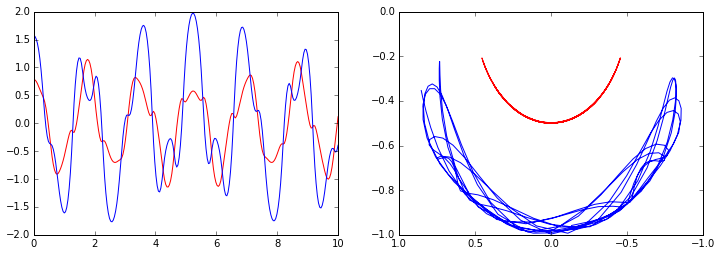
\includegraphics[width=\linewidth,keepaspectratio]{dblpend}
\end{center}
\end{frame}

%%%%%%%%%%%%%%%%%%%%%%%%%%%%%%%%%%%%%%%%%%%%%%%%%%%%%%%%%%%%%%%%%%%%%%%%%%%%%%%%%%
\begin{frame}[fragile]\frametitle{Fourier transform}
\begin{lstlisting}
from numpy.fft import fftfreq
from scipy.fftpack import *
N = len(t)
dt = t[1]-t[0]

# calculate the fast fourier transform
# y2 is the solution to the under-damped oscillator from the previous section
F = fft(y2[:,0]) 

# calculate the frequencies for the components in F
w = fftfreq(N, dt)
\end{lstlisting}
\end{frame}


%%%%%%%%%%%%%%%%%%%%%%%%%%%%%%%%%%%%%%%%%%%%%%%%%%%%%%%%%%%%%%%%%%%%%%%%%%%%%%%%%%
\begin{frame}[fragile]\frametitle{Fourier transform}
\begin{lstlisting}

fig, ax = plt.subplots(figsize=(9,3))
ax.plot(w, abs(F));
\end{lstlisting}
\begin{center}
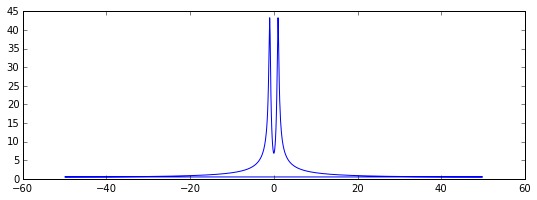
\includegraphics[width=\linewidth,keepaspectratio]{fft}
\end{center}
\end{frame}

%%%%%%%%%%%%%%%%%%%%%%%%%%%%%%%%%%%%%%%%%%%%%%%%%%%%%%%%%%%%%%%%%%%%%%%%%%%%%%%%%%
\begin{frame}[fragile]\frametitle{Linear algebra}
Linear equation systems on the matrix form $A x = b$
\begin{lstlisting}
from scipy.linalg import *
A = array([[1,2,3], [4,5,6], [7,8,9]])
b = array([1,2,3])
x = solve(A, b)

array([-0.33333333,  0.66666667,  0.        ])
\end{lstlisting}
\end{frame}

%%%%%%%%%%%%%%%%%%%%%%%%%%%%%%%%%%%%%%%%%%%%%%%%%%%%%%%%%%%%%%%%%%%%%%%%%%%%%%%%%%
\begin{frame}[fragile]\frametitle{Eigenvalues and eigenvectors}
The eigenvalue problem for a matrix $A$:
$A v_n = \lambda_n v_n$
\begin{lstlisting}
evals = eigvals(A)
array([ 1.08466629+0.j,  0.33612878+0.j, -0.28229973+0.j])

evals, evecs = eig(A)
array([ 1.08466629+0.j,  0.33612878+0.j, -0.28229973+0.j])
\end{lstlisting}
\end{frame}

%%%%%%%%%%%%%%%%%%%%%%%%%%%%%%%%%%%%%%%%%%%%%%%%%%%%%%%%%%%%%%%%%%%%%%%%%%%%%%%%%%
\begin{frame}[fragile]\frametitle{Matrix operations}
\begin{lstlisting}
# the matrix inverse
inv(A)

array([[ 2.0031935 , -0.63411453,  0.49891784],
       [-4.63643938, -0.2212669 ,  3.35170585],
       [ 1.06421936,  1.37366073, -1.42726809]])

# determinant
det(A)
-0.10292296739753022
       
\end{lstlisting}
\end{frame}

%%%%%%%%%%%%%%%%%%%%%%%%%%%%%%%%%%%%%%%%%%%%%%%%%%%%%%%%%%%%%%%%%%%%%%%%%%%%%%%%%%
\begin{frame}[fragile]\frametitle{Interpolation}
 \begin{itemize}
  \item  The interp1d function, when given arrays describing X and Y data, returns and object 
  \item It behaves like a function that can be called for an arbitrary value of x (in the range covered by X)
  \item It returns the corresponding interpolated y value.
   \end{itemize}
\begin{lstlisting}
from scipy.interpolate import *
def f(x):
    return sin(x)
n = arange(0, 10)  
x = linspace(0, 9, 100)

y_meas = f(n) + 0.1 * randn(len(n)) # simulate measurement with noise
y_real = f(x)

linear_interpolation = interp1d(n, y_meas)
y_interp1 = linear_interpolation(x)

cubic_interpolation = interp1d(n, y_meas, kind='cubic')
y_interp2 = cubic_interpolation(x)    
\end{lstlisting}
\end{frame}


%%%%%%%%%%%%%%%%%%%%%%%%%%%%%%%%%%%%%%%%%%%%%%%%%%%%%%%%%%%%%%%%%%%%%%%%%%%%%%%%%%
\begin{frame}[fragile]\frametitle{Interpolation}
\begin{lstlisting}
fig, ax = plt.subplots(figsize=(10,4))
ax.plot(n, y_meas, 'bs', label='noisy data')
ax.plot(x, y_real, 'k', lw=2, label='true function')
ax.plot(x, y_interp1, 'r', label='linear interp')
ax.plot(x, y_interp2, 'g', label='cubic interp')
ax.legend(loc=3);
\end{lstlisting}
\begin{center}
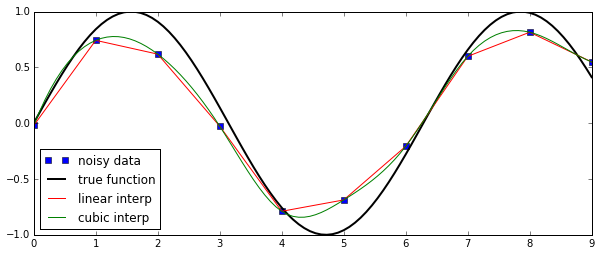
\includegraphics[width=\linewidth,keepaspectratio]{intpl}
\end{center}
\end{frame}

%%%%%%%%%%%%%%%%%%%%%%%%%%%%%%%%%%%%%%%%%%%%%%%%%%%%%%%%%%%%%%%%%%%%%%%%%%%%%%%%%%
\begin{frame}[fragile]\frametitle{Root finding using the bisection method}
\begin{lstlisting}
from scipy.optimize import bisect

def f(x):
    """returns f(x)=x^3-2x^2. Has roots at
    x=0 (double root) and x=2"""
    return x ** 3 - 2 * x ** 2

# main program starts here
x = bisect(f, 1.5, 3, xtol=1e-6)

print("The root x is approximately x=%14.12g,\n"
      "the error is less than 1e-6." % (x))
print("The exact error is %g." % (2 - x))

The root x is approximately x= 2.00000023842,
the error is less than 1e-6.
The exact error is -2.38419e-07.
\end{lstlisting}
\end{frame}


%%%%%%%%%%%%%%%%%%%%%%%%%%%%%%%%%%%%%%%%%%%%%%%%%%%%%%%%%%%%%%%%%%%%%%%%%%%%%%%%%%
\begin{frame}[fragile]\frametitle{Optimization}
\begin{lstlisting}
from scipy import optimize
def f(x):
    return x**2 + 10*np.sin(x)
    
grid = (-10, 10, 0.1)
xmin_global = optimize.brute(f, (grid,))
xmin_local = optimize.fminbound(f, 0, 10)
root = optimize.fsolve(f, 1)  # our initial guess is 1
root2 = optimize.fsolve(f, -2.5)
print xmin_global, xmin_local, root, root2

[-1.30641113] 3.8374671195 [ 0.] [-2.47948183]
\end{lstlisting}
\end{frame}


%%%%%%%%%%%%%%%%%%%%%%%%%%%%%%%%%%%%%%%%%%%%%%%%%%%%%%%%%%%%%%%%%%%%%%%%%%%%%%%%%%
\begin{frame}[fragile]\frametitle{Statistics}
\begin{lstlisting}
from scipy import stats
# create a (discreet) random variable with poissionian distribution

X = stats.poisson(3.5) # photon distribution for a coherent state with n=3.5 photons
n = arange(0,15)

fig, axes = plt.subplots(3,1, sharex=True)

# plot the probability mass function (PMF)
axes[0].step(n, X.pmf(n))

# plot the commulative distribution function (CDF)
axes[1].step(n, X.cdf(n))

# plot histogram of 1000 random realizations of the stochastic variable X
axes[2].hist(X.rvs(size=1000));
\end{lstlisting}
\begin{center}
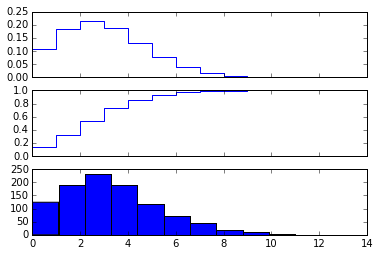
\includegraphics[width=0.5\linewidth,keepaspectratio]{poiss}
\end{center}
\end{frame}


%%%%%%%%%%%%%%%%%%%%%%%%%%%%%%%%%%%%%%%%%%%%%%%%%%%%%%%%%%%%%%%%%%%%%%%%%%%%%%%%%%
\begin{frame}[fragile]\frametitle{Statistics}
\begin{lstlisting}
# create a (continous) random variable with normal distribution
Y = stats.norm()
x = linspace(-5,5,100)

fig, axes = plt.subplots(3,1, sharex=True)

# plot the probability distribution function (PDF)
axes[0].plot(x, Y.pdf(x))

# plot the commulative distributin function (CDF)
axes[1].plot(x, Y.cdf(x));

# plot histogram of 1000 random realizations of the stochastic variable Y
axes[2].hist(Y.rvs(size=1000), bins=50);
\end{lstlisting}

\end{frame}

%%%%%%%%%%%%%%%%%%%%%%%%%%%%%%%%%%%%%%%%%%%%%%%%%%%%%%%%%%%%%%%%%%%%%%%%%%%%%%%%%%
\begin{frame}[fragile]\frametitle{Statistics}
\begin{center}
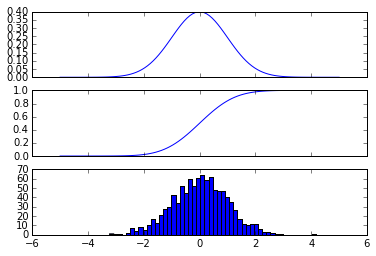
\includegraphics[width=\linewidth,keepaspectratio]{norm}
\end{center}
\end{frame}




